\subsubsection{Model reduction}\label{chapter_ModelReductionIMPL}

The already reduced process without the earthframe part, is not controllable (chapter \ref{chapter_controllabilityIMPL}). So there is need to reduce the model once again, but all remaining parts of the model are needed to construct the state space controller. In this stage, the reduced process has to be examined very carefully. Looking at the delay in the four motors of the process, reveals, that there is only one millisecond delay in each motor (figure \ref{fig:motorWithDelay}).

\begin{figure}
	\centering
		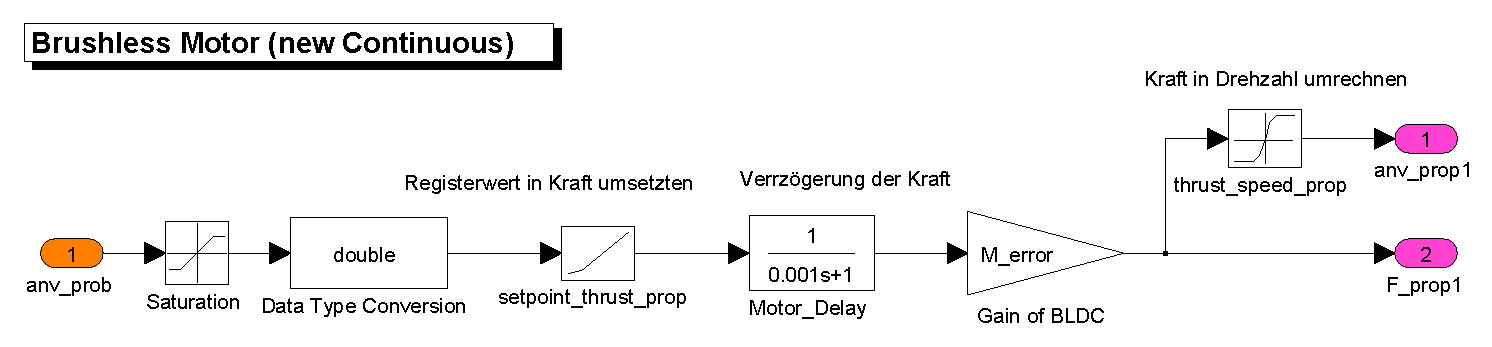
\includegraphics[width=1.00\textwidth]{03_Grafiken/motorWithDelay.pdf}
	\caption{Model of one motor including the time delay}
	\label{fig:motorWithDelay}
\end{figure}

In comprehension to the delays in each of the processes remaining integrators, the one millisecond can be disregarded (figure \ref{fig:motorWithoutDelay}). Now the same code, already used in chapter \ref{chapter_controllabilityIMPL}, has to run again, to check the controllability.

\begin{figure}
	\centering
		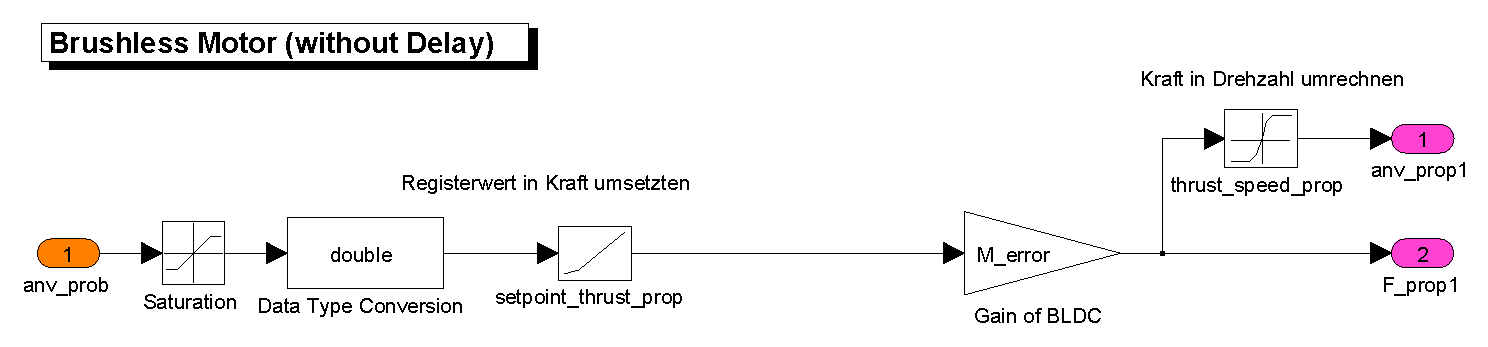
\includegraphics[width=1.00\textwidth]{03_Grafiken/motorWithoutDelay.pdf}
	\caption{Model of one motor without the time delay}		
	\label{fig:motorWithoutDelay}
\end{figure}


\begin{lstlisting}
	System = linmod('dynamics_reduced_without_motordelay');
	StateSpace = ss(System.a, System.b, System.c, System.d);
	rank(ctrb(StateSpace))  
	% ans = 5                 
\end{lstlisting}

Now the rank of the controllability matrix is five. That is the right number of controllable state variables, because the four motor delays are removed and so there are only five state variables remaining. At this point of the development it is not sure, if the state space controller, developed for this model without motor delay, will work later on with the process including the motor delay.
